\section{Definition}
Intuitively, if $x$ is a datapoint in a dataset $\D \subset \R^d$, a \emph{representation} of $x$ is a vector $r \in \R^n$ (usually, $n \leq d$), that shares information with the datapoint $x$. Representations are very often used in Machine Learning (ML).

Obtaining good representations of data is one of the most important tasks in ML. 
Recently, it has been discovered that maximizing the \emph{mutual information} between two elements in our data can give us good representations for our data.
In this section, \emph{information theory} notions will be presented, in order to use them in our ML models. This will provide a theoretical solid base for
the notions explained later.


The \emph{mutual information} concept is based on the \emph{Shannon entropy}, which we will introduce first, along with some basic properties of it. The Shannon entropy is a way of measuring the uncertainty in a random variable. 
Given an event $\mathcal A \in \Alg$, $P$ a probability measure and $P[\A]$ the probability of $\mathcal A$, we can affirm that 
$$
\log\frac{1}{P[\mathcal A]}
$$
describes \emph{"how surprising is that $\A$ occurs"}. Clearly, then, 
\begin{itemize}
\item If $P[\A]= 1$, then we have $\log 1 = 0$, which would indicate that it is not a surprise that $\A$ occurred.

\item On the other hand, if $P[A]\to 0$, then we have $\log(+\infty)$, which will surely be a big number indicating great surprise that $\A$ occurred.
\end{itemize}

With this motivation, we get to the following definition.
\begin{ndef}
Let $X$ be a discrete random variable with image $\X$. The \emph{Shannon entropy}, or simply \emph{entropy}  $H(X)$ of $X$ is defined as:
$$
H(X) = E_X\left[\log\frac{1}{P_X(X)}\right] =  \sum_{x \in \X} P_X(x) \log\frac{1}{P_X(x)}.
$$
\end{ndef}
The \emph{entropy} can trivially be expressed as:
$$
H(X) = - \sum_{x \in \X}P_X (x)\log P_X(x).
$$

This simple example, \citep{cover_elements_1991}, even though it is very simple, it is very illustrative for our definition:

%http://www.cs.columbia.edu/~vh/courses/LexicalSemantics/Association/Cover&Thomas-Ch2.pdf
\begin{nexample}
    \label{example:entropy}
Let $X \sim Bern(p)$. Then, the entropy of $X$ is:
\[
H(X) = -p \log p - (1-p) \log(1-p)) = H(p),
\]
since $H$ only depends on $p$. In Fig. \ref{example:entropy} we can see a representation of this function. We appreciate that in this case, $H$ is concave and equals $0$ if $p \in \{0,1\}$, which are the values of $p$ that give us no uncertainty. The maximum uncertainty is obtained when $p=\frac{1}{2}$, where we do not know what to expect as an outcome from our random variable $X$.

\begin{figure}[H]
    \label{fig:example:entropy}
    \centering
    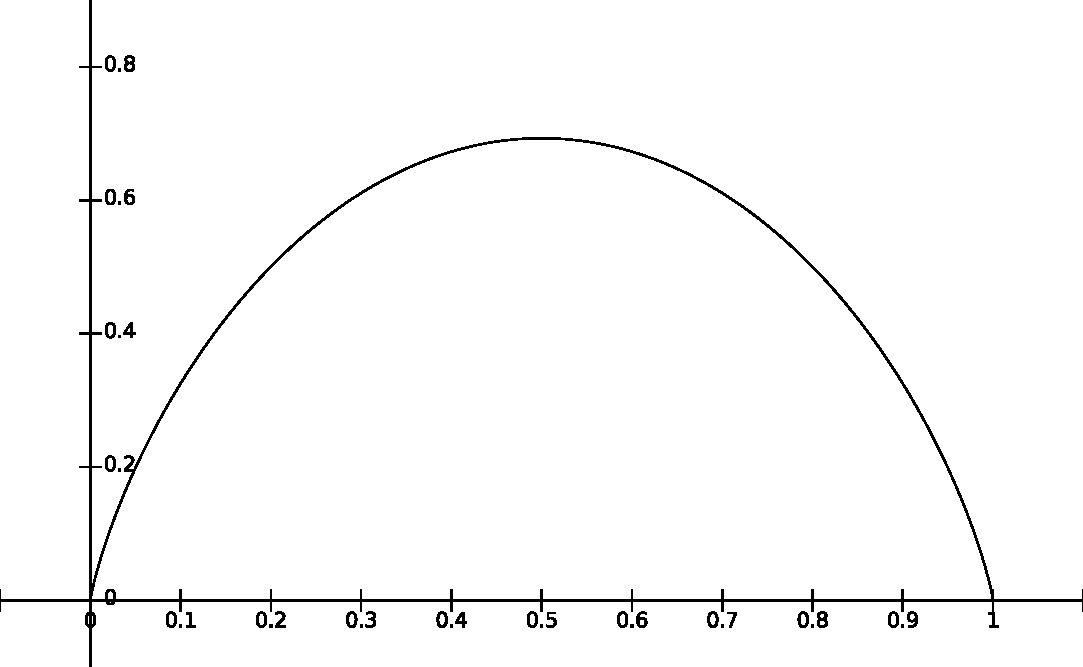
\includegraphics[scale=0.4]{Entropy.pdf}

      \caption{Representation of $H(p)$ in the example \ref{example:entropy}.}
\end{figure}

\end{nexample}
It can also be proven that, in general, the entropy is concave. 


\section{Properties of the entropy. Conditional entropy}

There are some properties of the \emph{entropy} that must be remarked, since they will extend to properties of the mutual information.


\begin{nprop}\label{entr:prop:1}
    Let $X$ be a random variable with image $\X$. If $|\X|$ is the cardinal of $\X$, then
    $$
0 \leq H(X) \leq \log(|\X|).
    $$
\end{nprop}
\begin{proof}
    Since $\log y$ is concave on $\R^+$, by Jensen's inequality ( see Appendix \ref{APPENDIX:A}, Prop. \ref{prop:jensen}), we obtain:
    $$
    H(X) = - \sum_{x \in \X}P_X (x)\log P_X(x) \leq \log\left(\sum_{x \in \X} 1\right) = \log(|\X|).
    $$
    For the lower bound we see that, since $P_X(x) \in [0,1]$ for all  $x \in \X $ then $\log P_X(x) \leq 0 \ \ \forall x \in \X$. Hence , $-P_X(x) \log P_X(x) \geq 0$ for all $x \in X$, so $H(X) \geq 0$.
\end{proof}
We can also see that the equality on the left holds if , and only if , exists $ x $ in  $X$ such that its probability is exactly one, that is $P_X(x) = 1$. The right equality holds if and only if , for all $x \in \X$, its probability is $P_X(x) = \frac{1}{\abs{X}}$.

\subsection*{Conditional entropy}
We have already said that entropy measures how surprising is that an event occurs.
Usually, we will be looking at two random variables and it would be interesting to see how likely is that one of them, say $X(x)$, occurred, if we already know that $Y(y)$ occurred. 
This leads us to the definition of \emph{conditional entropy}. Let us see a simpler case first:

Let $A$ be an event, and $X$ a random variable. The conditional probability $P_{X|A}$ defines the entropy of $X$ conditioned to $ A$:
$$
H(X| A) = \sum_{x \in \X} P_{X|A}(x) \log\frac{1}{P_{X|A}(x)}.
$$
If $Y$ is another random variable and $\mathcal Y$ is its image, intuitively we can sum the conditional entropy of an event with all the events in $\mathcal Y$, and this way we obtain the conditional entropy of $X$ given $Y$.
\begin{ndef}[Conditional Entropy]
Let $X,Y$ be random variables with images $\X,\mathcal Y$. The \emph{conditional entropy} $H(X | Y)$ is defined as:

\begin{equation*}
    \begin{split}
    H(X|Y) &  :=   \sum_{y \in \mathcal Y} P_{\mathcal Y}(y) H(X| Y = y)  \\ 
    & = \sum_{y \in \mathcal Y} P_{\mathcal  Y}(y) \sum_{x \in \X} P_{X | Y}(x|y)\log\frac{1}{P_{X|Y}(x|y)}  \\
   & = \sum_{x \in X,y \in \mathcal Y}P_{XY}(x,y)\log\frac{P_Y(y)}{P_{XY}(x,y)}.
\end{split}
\end{equation*}
\end{ndef}

The interpretation of the conditional entropy is simple: the uncertainty in $X$ when $Y$ is given.
Since we know about an event that has occurred ($Y$), intuitively the conditional entropy , or the uncertainty of $X$ occurring given that $Y$ has occurred, will be lesser than the entropy of $X$, since we already have some information about what is happening. We can prove this:

\begin{nprop}\label{entr:prop:2}
Let $X,Y$ be random variables with images $\mathcal X, \mathcal Y$. Then:
$$
0 \leq H(X|Y) \leq H(X).
$$
\end{nprop}
\begin{proof}

The inequality on the left was proved on Proposition \ref{entr:prop:1}. The characterization of when $H(X|Y) = 0$ was also mentioned after it.
Let us look at the inequality on the right. Note that restricting to the $(x,y)$ where $P_{XY}(x,y) > 0$ and using the definition of the conditional probability we have:
\begin{align*}
H(X|Y) = & \sum_{y \in \mathcal{Y}} P_Y(y) \sum_{x \in \X} P_{X|Y}(x|y)\log \frac{1}{P_{X|Y}(x|y)}\\
 = & \sum_{x \in \mathcal X,y \in \mathcal Y} P_Y(y) P_{X|Y}(x,y) \log \frac{P_Y(y)}{P_{XY}(x,y)} \\
  = & \sum_{x \in \mathcal X,y \in \mathcal Y} P_{XY}(x,y)\log \frac{P_Y(y)}{P_{XY}(x,y)} ,
\end{align*}
and 
$$
H(X) = \sum_x P_X(x) \log \frac{1}{P_X(x)} = \sum_{x,y}P_{XY}(x,y) \log \frac{1}{P_X(x)}.
$$
Hence,
\begin{equation}\label{eq:dif-expr-mi}
\begin{split}
H(X|Y) - H(X) = & \sum_{x,y}P_{XY}(x,y) \left( \log \frac{P_Y(y)}{P_{XY}(x,y)} - \log \frac{1}{P_X(x)}\right) \\ 
= &  \sum_{x,y}P_{XY}\log \frac{P_Y(y)P_X(x)}{P_{XY}(x,y)}.
\end{split}
\end{equation}
So, using Jensen's inequality, we obtain:
\begin{align*}
\sum_{x,y}P_{XY}\log \frac{P_Y(y)P_X(x)}{P_{XY}(x,y)} \leq & \log \left( \sum_{x,y}\frac{ \cancel{P_{XY}(x,y)} \ \  P_Y(y) P_X(x)}{\cancel{P_{XY}(x,y)}} \right) \\ 
= & \log\left( \left( \sum_x P_X(x) \right) \left(\sum_y P_Y(y)\right)\right) = \log 1 = 0,
\end{align*}
and this leads us to:
\begin{equation}\label{prop:2:2nd:ineq}
H(X|Y) - H(X) \leq 0 \quad \text{ then } \quad H(X|Y) \leq H(X)
\end{equation}
as we wanted.
\end{proof}

It must be noted that the inequality the state of the proposition,
$$
0 \leq H(X|Y) \leq H(X),
$$

in the inequality of the left, equality holds if, and only if, $P_{XY}(x,y) = P_X(x) P_Y(y)$ for all $(x,y)$ with $P_{XY} (x,y) > 0$, as it is said in Jensen's inequality.
For the inequality on the right, equality holds if and only if $P_{XY}(x,y) = 0$, which implies $P_X(x)P_Y(y) = 0$ for any $x\in \mathcal X$, $y \in \mathcal Y$. It follows that $H(X|Y) = H(X)$ if and only if $P_{XY}(x,y) = P_X(x)P_Y(y)$ for all $(x,y) \in \mathcal X \times \mathcal Y$

